\documentclass[10 pt]{article}
\usepackage{graphicx}
\pagestyle{plain}
\usepackage[OT4]{polski}
\usepackage[utf8]{inputenc}
\title{Sprawozdzanie 3\\ \emph{\textbf{Porównanie czasów wypełniania stosu/kolejki za pomocą
tablicy/listy }}}
\author{Paweł Żurek 200404}
\date{20.03.2014}
\begin{document}
\tableofcontents
\maketitle
\section{Wstep}
\textbf{Program porównuje czasy wypełniania następujących struktur : }
\begin{itemize}
\item Stosu za pomocą :
\begin{itemize}
\item tablicy
\item listy
\end{itemize}
\item Kolejki za pomocą :
\begin{itemize}
\item tablicy
\item listy
\end{itemize}
\end{itemize}

\section{Wyniki}

\paragraph{Wynik działania programu  : \\}
\begin{center}
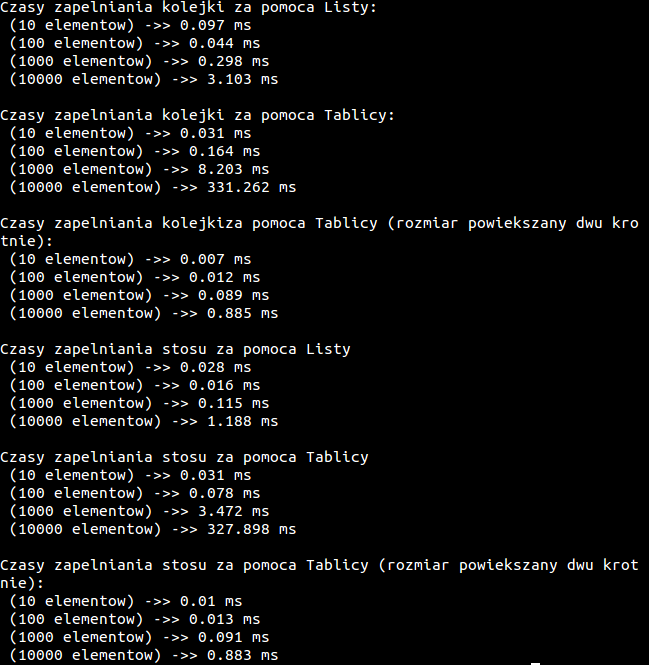
\includegraphics[scale=0.5]{dzialanie.png}
\end{center}
\newpage
\paragraph{Dane wyświetlone za pomoca wykresu ( wykres dostępny osobno w pliku wykres.pdf) }
\begin{center}
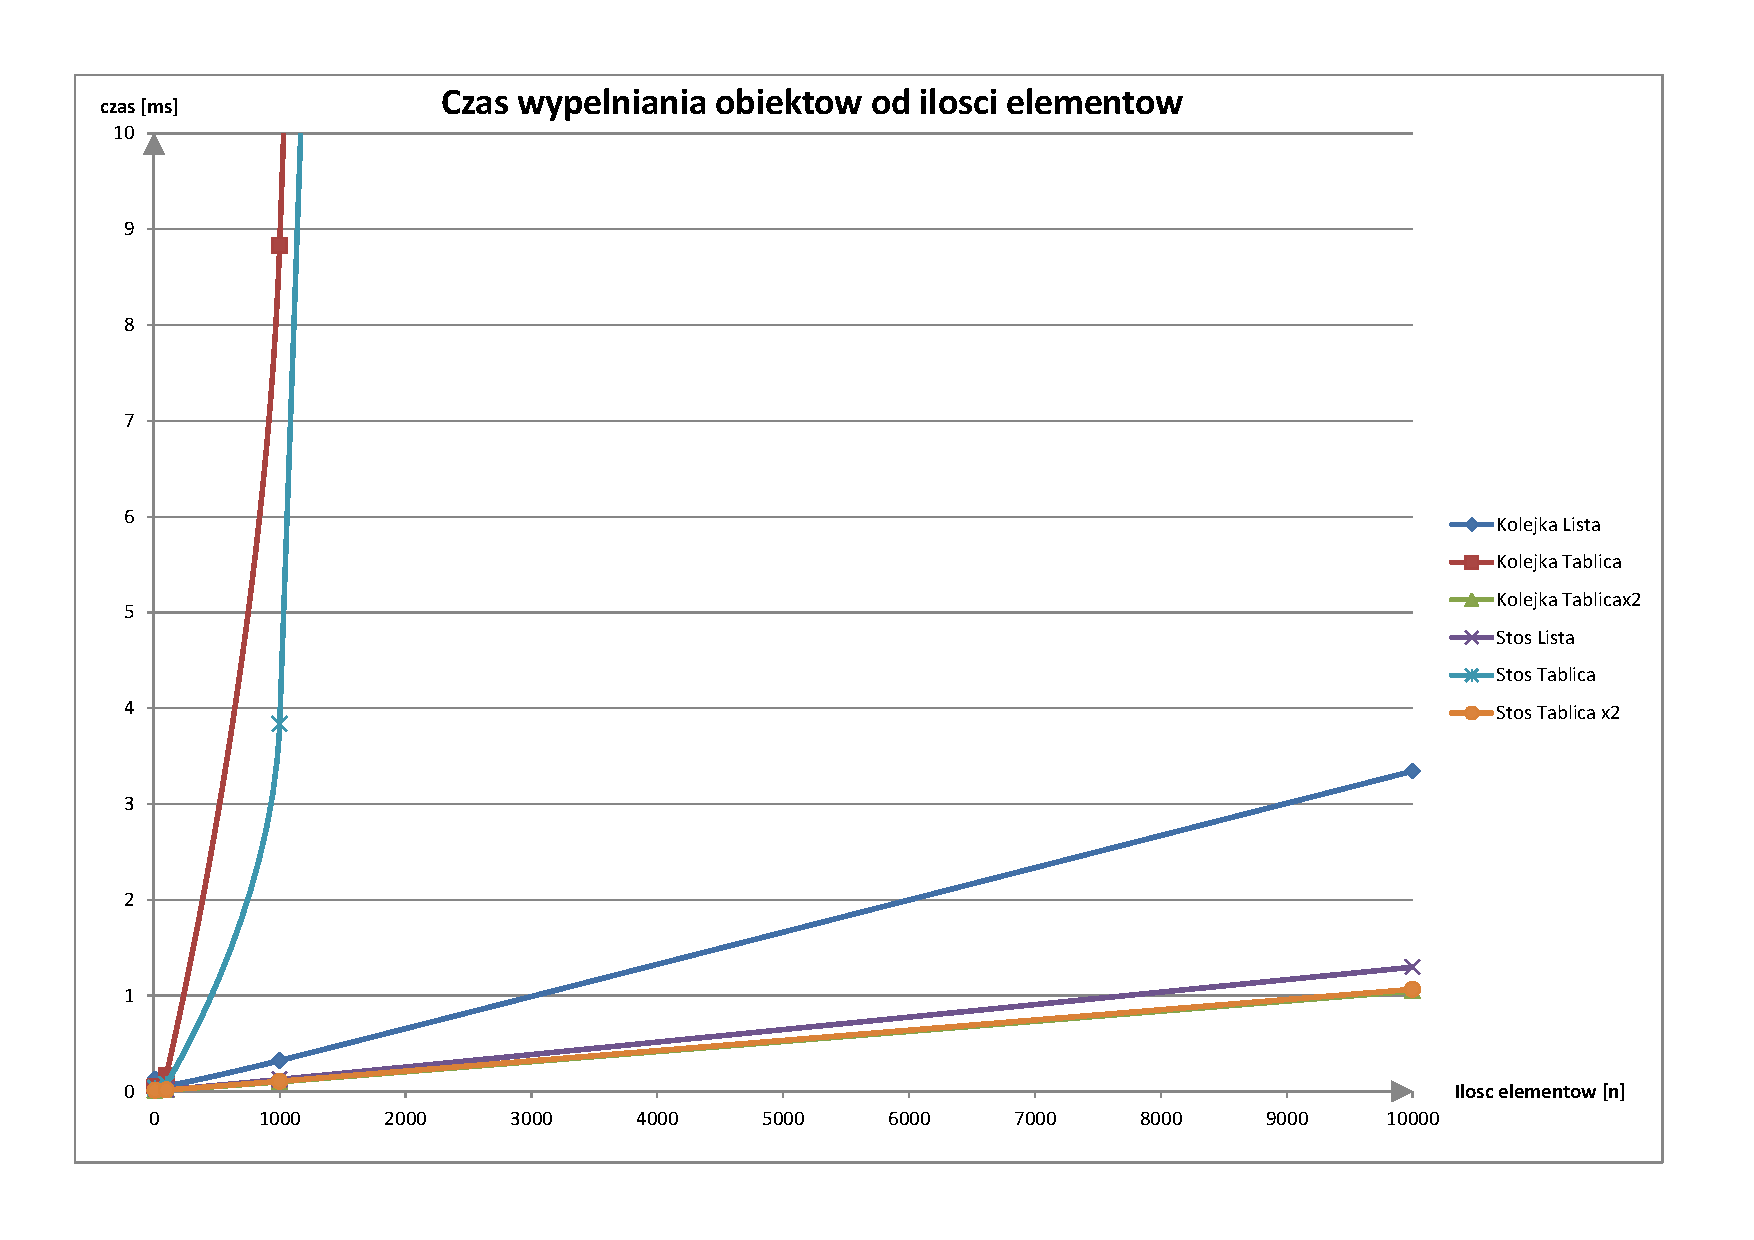
\includegraphics[scale=0.4]{wykres.pdf}
\end{center}

\section{Wnioski:}
\begin{itemize}
\item W każdym przypadku wypełnianie stosu okazało się szybsze niż wypełnianie kolejki
\item Wypełnianie obiektów za pomocą tablicy, która powiększa swój rozmiar o jeden jest zdecydowanie
najwolniejszym sposobem
\item Natomiast najszybszym sposobem jest wypełnianie obiektów za pomocą tablicy, która powiększa
swój rozmiar dwa razy przy przekroczeniu aktualnego rozmiaru. Dzieje się tak, ponieważ
zwiększając swój rozmiar dwa razy, liczba usunięć i ponownych zaalokowań tablicy jest
zdecydowanie więcej
\item Wypełnianie obiektów listą stosu jak i kolejki jest podobne, jest również bardzo zbliżone do
najszybszego sposobu. Ciekawe jest to, że w obu przypadkach listy dziesięcioma elementami trwa
dużej niż zapełnienie tej samej listy stu elementami.
\end{itemize}
Dokumentacja program dostępna w pliku pdf o nazwie ''Dokumentacja'' (zapisana w \LaTeX u) oraz w DoxyGen'ie (dostępna w pliku : dox/html/index.html)

\end{document}